%%%%%%%%%%%%%%%%%%%%%%%%%%%%%%%%%%%%%%%%%%%%%%%%%%%%%%%%%%%%%%%%%%%%%%%%%%%%%%%
% Robust Control Course Project — Presentation slides
% LQR vs LQR+DOB for differential-drive mobile robot trajectory tracking
%
% Compile with:  pdflatex slides && pdflatex slides
% (or use latexmk -pdf slides.tex)
%
% Theme: metropolis (modern, minimal). If your TeX installation lacks
% metropolis, comment out lines 14-15 and uncomment the Madrid fallback.
%%%%%%%%%%%%%%%%%%%%%%%%%%%%%%%%%%%%%%%%%%%%%%%%%%%%%%%%%%%%%%%%%%%%%%%%%%%%%%%

\documentclass[10pt,aspectratio=169]{beamer}

% ---------- theme ----------
\usetheme{metropolis}
\metroset{block=fill,sectionpage=progressbar,subsectionpage=progressbar}

% ---------- fallback theme (uncomment if metropolis not available) ----------
% \usetheme{Madrid}
% \usecolortheme{whale}

% ---------- packages ----------
\usepackage[utf8]{inputenc}
\usepackage{amsmath,amssymb,amsfonts,bm,mathtools}
\usepackage{booktabs,multirow,array}
\usepackage{graphicx,subcaption}
\usepackage{tikz}
\usepackage{xcolor}
\usepackage{appendixnumberbeamer}

\usetikzlibrary{positioning,arrows.meta,calc,decorations.pathmorphing}

% ---------- custom commands ----------
\newcommand{\R}{\mathbb{R}}
\newcommand{\norm}[1]{\left\lVert#1\right\rVert}
\definecolor{accent}{RGB}{200,80,30}
\definecolor{accent2}{RGB}{30,80,180}

%%%%%%%%%%%%%%%%%%%%%%%%%%%%%%%%%%%%%%%%%%%%%%%%%%%%%%%%%%%%%%%%%%%%%%%%%%%%%%%
\title{Robust Trajectory Tracking of a Mobile Robot}
\subtitle{LQR with Disturbance-Observer Compensation}
\author[Peng, Yang, Lu]{Jianwei Peng \and Han Yang \and Ziling Lu}
\institute{Department of Automation, SUSTech}
\date{Robust Control Course Project, 2026}

%%%%%%%%%%%%%%%%%%%%%%%%%%%%%%%%%%%%%%%%%%%%%%%%%%%%%%%%%%%%%%%%%%%%%%%%%%%%%%%
\begin{document}

% ============================== Title ============================== %
\begin{frame}[plain]
  \titlepage
\end{frame}

% ============================== Outline ============================ %
\begin{frame}{Outline}
  \tableofcontents[hideallsubsections]
\end{frame}

%%%%%%%%%%%%%%%%%%%%%%%%%%%%%%%%%%%%%%%%%%%%%%%%%%%%%%%%%%%%%%%%%%%%%%%%%%%%%%%
\section{Motivation}

\begin{frame}{The trajectory-tracking problem}
  \begin{columns}[T]
    \column{0.55\linewidth}
      \textbf{Differential-drive mobile robot} (WMR)
      \begin{itemize}
        \item Pose $q=(x,y,\theta)$, velocity $\eta=(v,\omega)$
        \item Nonholonomic, nonlinearly coupled
        \item Must track a time-parameterised reference path
      \end{itemize}

      \vspace{0.4em}
      \textbf{Sources of error}
      \begin{itemize}
        \item Exogenous torque disturbance $\tau_d$ (slip, terrain)
        \item Parametric drift in $(m, I, d_v, d_\omega)$
              (payload change, wear)
        \item Sensor noise
      \end{itemize}

      \vspace{0.4em}
      \alert{Question:} can a single LQR controller handle all of
      these robustly?

    \column{0.45\linewidth}
      \centering
      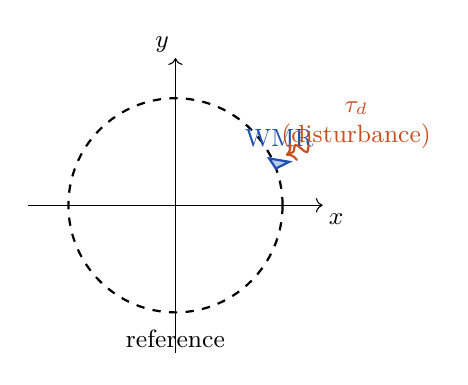
\begin{tikzpicture}[scale=0.85, every node/.style={font=\small}]
        % reference circle
        \draw[dashed,thick] (0,0) circle (1.6);
        \node at (0,-2.0) {reference};
        % robot
        \draw[fill=accent2!30,draw=accent2,thick]
              (1.4,0.7) -- (1.7,0.65) -- (1.5,0.55) -- cycle;
        \node[accent2] at (1.55,1.0) {WMR};
        % disturbance arrow
        \draw[->,thick,accent,decorate,
              decoration={snake,amplitude=0.7mm,segment length=2mm}]
              (2.0,0.9) -- (1.65,0.75);
        \node[accent,align=center] at (2.7,1.2)
              {$\tau_d$\\(disturbance)};
        % axes
        \draw[->] (-2.2,0) -- (2.2,0);
        \draw[->] (0,-2.2) -- (0,2.2);
        \node at (2.4,-0.2) {$x$}; \node at (-0.2,2.4) {$y$};
      \end{tikzpicture}
  \end{columns}
\end{frame}

\begin{frame}{Why plain LQR is not enough}
  \begin{columns}[T]
    \column{0.55\linewidth}
      \textbf{Plain LQR} on the linearised error model
      \begin{itemize}
        \item Optimal for the \emph{nominal} system
        \item No internal model of $\tau_d$
        \item $\Rightarrow$ steady-state offset under any
              persistent disturbance
      \end{itemize}

      \vspace{0.6em}
      \textbf{Concrete demonstration} (right):\\
      step disturbance
      $\tau_d=(0.5,0.15)$\,N$\cdot$m at $t=8$\,s
      \begin{itemize}
        \item LQR settles at $\sim 0.11$\,m \alert{persistent error}
        \item LQR+DOB recovers to zero in $\approx 4$\,s
      \end{itemize}

      \vspace{0.6em}
      \alert{Goal of this work:} retain LQR's optimal nominal behaviour
      but add an internal model so disturbances are cancelled online.

    \column{0.45\linewidth}
      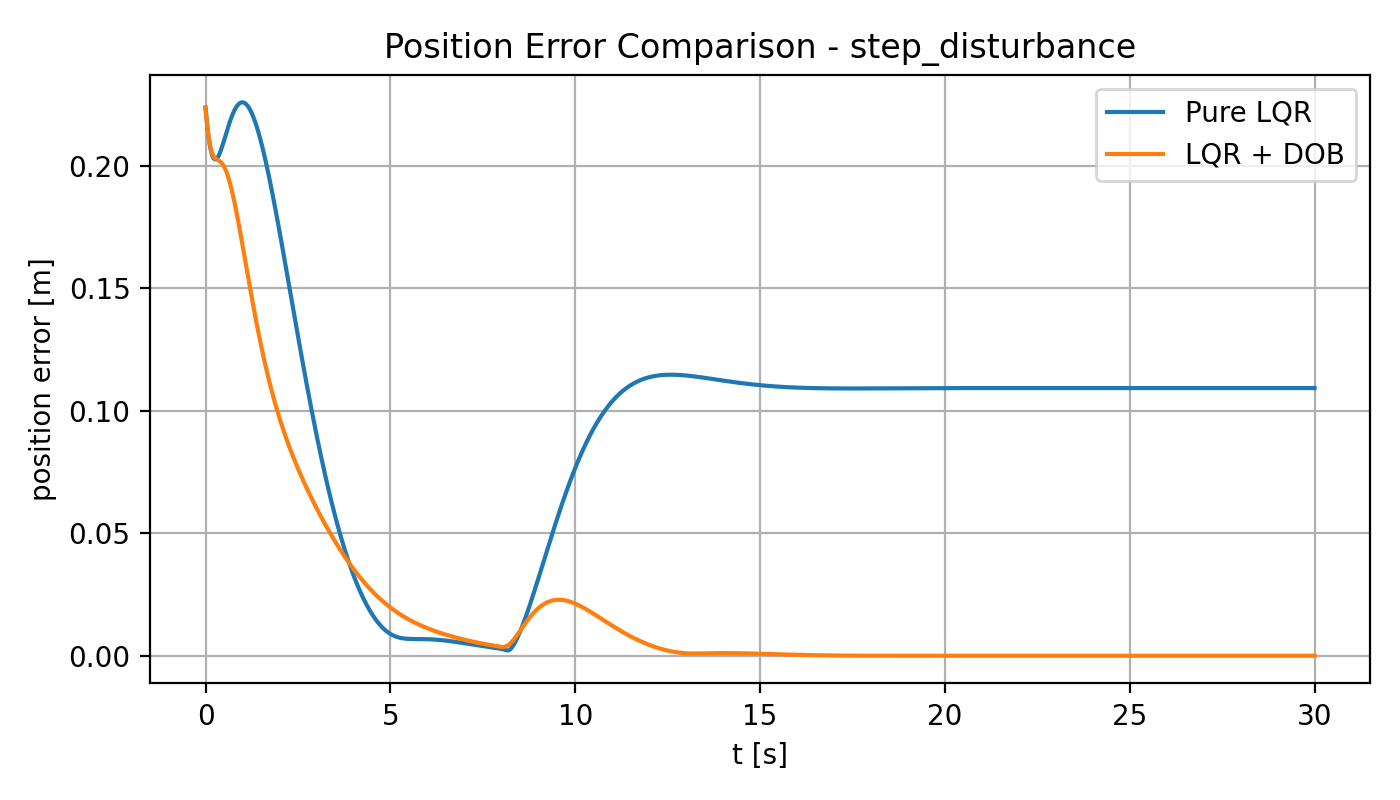
\includegraphics[width=\linewidth]{figs/step_disturbance_position_error_compare.png}
      \vspace{-0.4em}
      \begin{center}\scriptsize Position error under step disturbance.\end{center}
  \end{columns}
\end{frame}

%%%%%%%%%%%%%%%%%%%%%%%%%%%%%%%%%%%%%%%%%%%%%%%%%%%%%%%%%%%%%%%%%%%%%%%%%%%%%%%
\section{Related Work}

\begin{frame}{Spectrum of robust controllers}
  \begin{center}\small
  \begin{tabular}{lll}
    \toprule
    Approach & Strength & Limitation\\
    \midrule
    LQR \cite{kanayama1990}        & Optimal, simple   & No disturbance rejection\\
    DOBC \cite{ohnishi1996,chen2016}& Cancels matched $d$ & Needs internal model\\
    SMC \cite{utkin2013}           & Robust to bounded unc. & Chattering\\
    $H_\infty$ \cite{zhou1996}     & Worst-case bound  & Conservative, complex\\
    Tube-MPC \cite{mayne2005}      & Constraints, robust & Computation\\
    \bottomrule
  \end{tabular}
  \end{center}

  \vspace{0.6em}
  \textbf{Our choice: LQR + DOB.} A pragmatic balance
  \begin{itemize}
    \item Keeps LQR's closed-form optimality
    \item Adds a Luenberger observer with explicit pole-placement rule
    \item Provable stability under time-scale separation
  \end{itemize}
\end{frame}

%%%%%%%%%%%%%%%%%%%%%%%%%%%%%%%%%%%%%%%%%%%%%%%%%%%%%%%%%%%%%%%%%%%%%%%%%%%%%%%
\section{System Model}

\begin{frame}{Differential-drive dynamics}
  \textbf{Kinematics} (world frame):
  \begin{equation*}
    \dot q=\begin{bmatrix}\cos\theta & 0\\ \sin\theta & 0\\ 0 & 1\end{bmatrix}\eta,
    \qquad q=\begin{bmatrix}x\\y\\\theta\end{bmatrix},\ \eta=\begin{bmatrix}v\\\omega\end{bmatrix}
  \end{equation*}

  \textbf{Body-frame dynamics}:
  \begin{equation*}
    M_0\dot\eta+D_0\eta=\tau+\tau_d
  \end{equation*}
  with $M_0=\mathrm{diag}(m_0,I_0)$, $D_0=\mathrm{diag}(d_{v0},d_{\omega 0})$.

  \vspace{0.5em}
  \textbf{Parametric uncertainty} modelled as
  \begin{equation*}
    M(t)=M_0+\Delta M(t),\qquad D(t)=D_0+\Delta D(t).
  \end{equation*}

  \vspace{0.4em}
  \textbf{Reference:} circular path with constant
  $v_r=R_c\Omega,\ \omega_r=\Omega$.

  \vspace{0.4em}
  Nominal values for this study:
  $m_0\!=\!5\,\mathrm{kg}, I_0\!=\!0.5\,\mathrm{kg\,m^2}, d_{v0}\!=\!1, d_{\omega 0}\!=\!0.5$,
  $R_c\!=\!2\,\mathrm{m}, \Omega\!=\!0.2\,\mathrm{rad/s}$.
\end{frame}

\begin{frame}{Tracking error and linearisation}
  \textbf{Body-frame tracking error}
  \begin{equation*}
    \xi=\begin{bmatrix}x_e\\y_e\\\theta_e\\v_e\\\omega_e\end{bmatrix}
       =\begin{bmatrix}
       \hphantom{-}\cos\theta(x_r{-}x)+\sin\theta(y_r{-}y)\\
       -\sin\theta(x_r{-}x)+\cos\theta(y_r{-}y)\\
       \mathrm{wrap}(\theta_r-\theta)\\ v_r-v\\ \omega_r-\omega
       \end{bmatrix}
  \end{equation*}

  \textbf{Linearisation around} $\xi=0$ with feed-forward $\tau_{ff}$:
  \begin{equation*}
    \dot\xi = A\xi + B(u + d)
  \end{equation*}
  where $d$ is the \alert{matched equivalent disturbance} — the projection of
  all model mismatch and $\tau_d$ onto the input channel.

  \vspace{0.3em}
  \begin{block}{Numerical matrices for our parameters}
    \[ A=\!\begin{bmatrix}
       0 & 0.2 & 0 & 1 & 0\\
       -0.2 & 0 & 0.4 & 0 & 0\\
       0 & 0 & 0 & 0 & 1\\
       0 & 0 & 0 & -0.2 & 0\\
       0 & 0 & 0 & 0 & -1
    \end{bmatrix}\!,\;
    B=\!\begin{bmatrix}
       0 & 0\\0 & 0\\0 & 0\\0.2 & 0\\0 & 2
    \end{bmatrix} \]
    $\mathrm{rank}\,\mathcal{C}=5$ \ $\Rightarrow$ \ fully controllable.
  \end{block}
\end{frame}

%%%%%%%%%%%%%%%%%%%%%%%%%%%%%%%%%%%%%%%%%%%%%%%%%%%%%%%%%%%%%%%%%%%%%%%%%%%%%%%
\section{Controller Design}

\begin{frame}{Step 1 — Baseline LQR}
  \textbf{Quadratic cost} (ignoring $d$):
  \begin{equation*}
    J=\int_0^\infty\Bigl(\xi^\top Q\xi+u^\top Ru\Bigr)dt,\quad
    Q\succeq 0,\ R\succ 0.
  \end{equation*}

  \textbf{HJB} $\rightarrow$ \textbf{Continuous algebraic Riccati equation}:
  \begin{equation*}
    A^\top P+PA-PBR^{-1}B^\top P+Q=0,
    \quad u_{\mathrm{LQR}}=-K\xi,\quad K=R^{-1}B^\top P.
  \end{equation*}

  \vspace{0.4em}
  \textbf{Design choice}: $Q=\mathrm{diag}(20,20,10,2,2),\ R=I_2$.

  \vspace{0.3em}
  \begin{block}{Closed-loop spectrum (computed)}
    \centering
    $\sigma(A-BK)=\{-2.28\!\pm\!j0.94,\ -0.68\!\pm\!j0.68,\ -0.61\}$
  \end{block}

  \vspace{0.2em}
  \alert{Hurwitz} $\Rightarrow$ nominal asymptotic stability. \
  Slowest rate
  $\alpha\!=\!|\mathrm{Re}\,\lambda_{\min}|\!\approx\!0.61$ — used to size
  the observer next.
\end{frame}

\begin{frame}{Step 2 — Augmented-state disturbance observer}
  \textbf{Internal model of $d$:} treat $\dot d=0$. Augment the state
  $x_a=(\xi,d)\in\R^7$:
  \begin{equation*}
    \dot x_a=\underbrace{\begin{bmatrix}A & B\\ 0 & 0\end{bmatrix}}_{A_a}
              x_a +
              \underbrace{\begin{bmatrix}B\\0\end{bmatrix}}_{B_a}u,
    \quad y=C_a x_a=\xi
  \end{equation*}

  Observability check: $\mathrm{rank}\,\mathcal{O}_a=7$\ \checkmark.

  \vspace{0.5em}
  \textbf{Luenberger observer}:
  \begin{equation*}
    \dot{\hat x}_a=A_a\hat x_a+B_a u+L(y-C_a\hat x_a)
  \end{equation*}

  \textbf{Composite control law}:
  \begin{equation*}
    \boxed{u=-K\xi-\hat d}
  \end{equation*}
  — LQR for tracking, $-\hat d$ for disturbance cancellation.
\end{frame}

\begin{frame}{Step 3 — Observer pole placement}
  \textbf{Time-scale separation rule}: observer must be faster than LQR.
  \begin{equation*}
    \lambda_i^{\mathrm{obs}}=-\rho\,\alpha\,\mu_i,
    \quad i=1,\ldots,7
  \end{equation*}
  \begin{itemize}
    \item $\alpha=|\mathrm{Re}\,\lambda_{\min}(A_K)|\approx 0.61$
          (slowest LQR rate)
    \item $\rho>1$: \alert{speed factor} (user-tunable)
    \item $\{\mu_i\}=\{1.00,1.15,1.30,1.50,1.75,2.05,2.40\}$
          (Butterworth spacing, avoids coincident poles)
  \end{itemize}

  \vspace{0.4em}
  Gain $L\in\R^{7\times 5}$ obtained via Tits--Yang multivariable pole
  placement~\cite{kautsky1985} (\texttt{scipy.signal.place\_poles}).

  \vspace{0.5em}
  \textbf{For $\rho=5$}: observer poles lie in $[-7.31,-3.05]$\,---
  \alert{$\sim 5\times$ faster} than the LQR closed loop. \
  (Trade-off explored in slides 14-15.)
\end{frame}

%%%%%%%%%%%%%%%%%%%%%%%%%%%%%%%%%%%%%%%%%%%%%%%%%%%%%%%%%%%%%%%%%%%%%%%%%%%%%%%
\section{Stability Analysis}

\begin{frame}{Closed-loop dynamics and Theorem 1}
  Substituting $u=-K\xi-\hat d$ and $e=x_a-\hat x_a$:
  \begin{equation*}
    \begin{aligned}
      \dot\xi &= A_K\xi + B\,e_d  & \text{(tracking error)}\\
      \dot e   &= (A_a-LC_a)\,e    & \text{(observer error)}
    \end{aligned}
  \end{equation*}
  — a \alert{cascade} of two Hurwitz subsystems.

  \begin{block}{Theorem 1 (stability of the cascade)}
    Under stabilisability of $(A,B)$, observability of $(A_a,C_a)$, and the
    observer rule with any $\rho>1$:
    \begin{enumerate}
      \item[(i)] for constant $d$, $(\xi,e)\to 0$ \emph{exponentially};
      \item[(ii)] for $\norm{\dot d}\le\delta$, the cascade is UUB with
                  ultimate bound $O(\delta/\rho)$.
    \end{enumerate}
  \end{block}

  \textbf{Implication:} larger $\rho$ tightens the steady-state bound but
  amplifies noise — matches the empirical sweep.
\end{frame}

\begin{frame}{Proof sketch}
  Composite Lyapunov function
  \begin{equation*}
    V(\xi,e)=\xi^\top P_\xi\xi+\beta\,e^\top P_e e,
    \quad\beta>0.
  \end{equation*}
  where $P_\xi,P_e\succ 0$ solve the respective Lyapunov equations.

  Differentiating along the closed loop (constant $d$):
  \begin{equation*}
    \dot V=-\norm\xi^2+2\xi^\top P_\xi B e_d-\beta\norm e^2.
  \end{equation*}
  Young's inequality with $\epsilon=1/2$ and $\beta>2\norm{P_\xi B}^2$:
  \begin{equation*}
    \dot V\le-\tfrac12\norm\xi^2-c_e\norm e^2\le-\gamma V,\quad
    \gamma>0.
  \end{equation*}
  $\Rightarrow$ exponential stability of the cascade. \hfill $\square$

  \vspace{0.6em}
  Time-varying $d$ adds a $\dot d$-driven perturbation;
  $\norm{P_e}=O(1/\rho)$ gives ultimate bound $O(\delta/\rho)$.
\end{frame}

%%%%%%%%%%%%%%%%%%%%%%%%%%%%%%%%%%%%%%%%%%%%%%%%%%%%%%%%%%%%%%%%%%%%%%%%%%%%%%%
\section{Simulation Results}

\begin{frame}{Simulation setup}
  \begin{columns}[T]
    \column{0.5\linewidth}
      \textbf{Plant:} full nonlinear model integrated with RK45\\
      ($\mathtt{rtol}{=}10^{-7}$, $\mathtt{atol}{=}10^{-9}$,\\
       $T{=}30$\,s, $\mathrm{d}t{=}0.02$\,s)

      \vspace{0.6em}
      \textbf{Initial pose:} $(2.2,\,0.1,\,\pi/2)$ — off-track
      by $\approx 0.22$\,m

      \vspace{0.6em}
      \textbf{Controllers compared:}
      \begin{itemize}
        \item Plain LQR
        \item LQR + DOB with $\rho=5$
      \end{itemize}

    \column{0.5\linewidth}
      \textbf{Five scenarios:}
      \begin{enumerate}\setlength\itemsep{2pt}
        \item[(S1)] Nominal (no disturbance)
        \item[(S2)] Step $\tau_d{=}(0.5,0.15)$ at $t{=}8$\,s
        \item[(S3)] Piecewise $\tau_d$ — switches at 5/10/15\,s
        \item[(S4)] Payload $\Delta m{=}10$, $\Delta I{=}0.8$ at $t{=}5$\,s
        \item[(S5)] Noisy $\tau_d$ + friction perturbation
      \end{enumerate}
  \end{columns}

  \vspace{0.6em}
  \centering
  \alert{Same $K$, $L$ used across all scenarios — no per-case tuning.}
\end{frame}

\begin{frame}{Trajectory tracking under piecewise disturbance (S3)}
  \begin{columns}[T]
    \column{0.55\linewidth}
      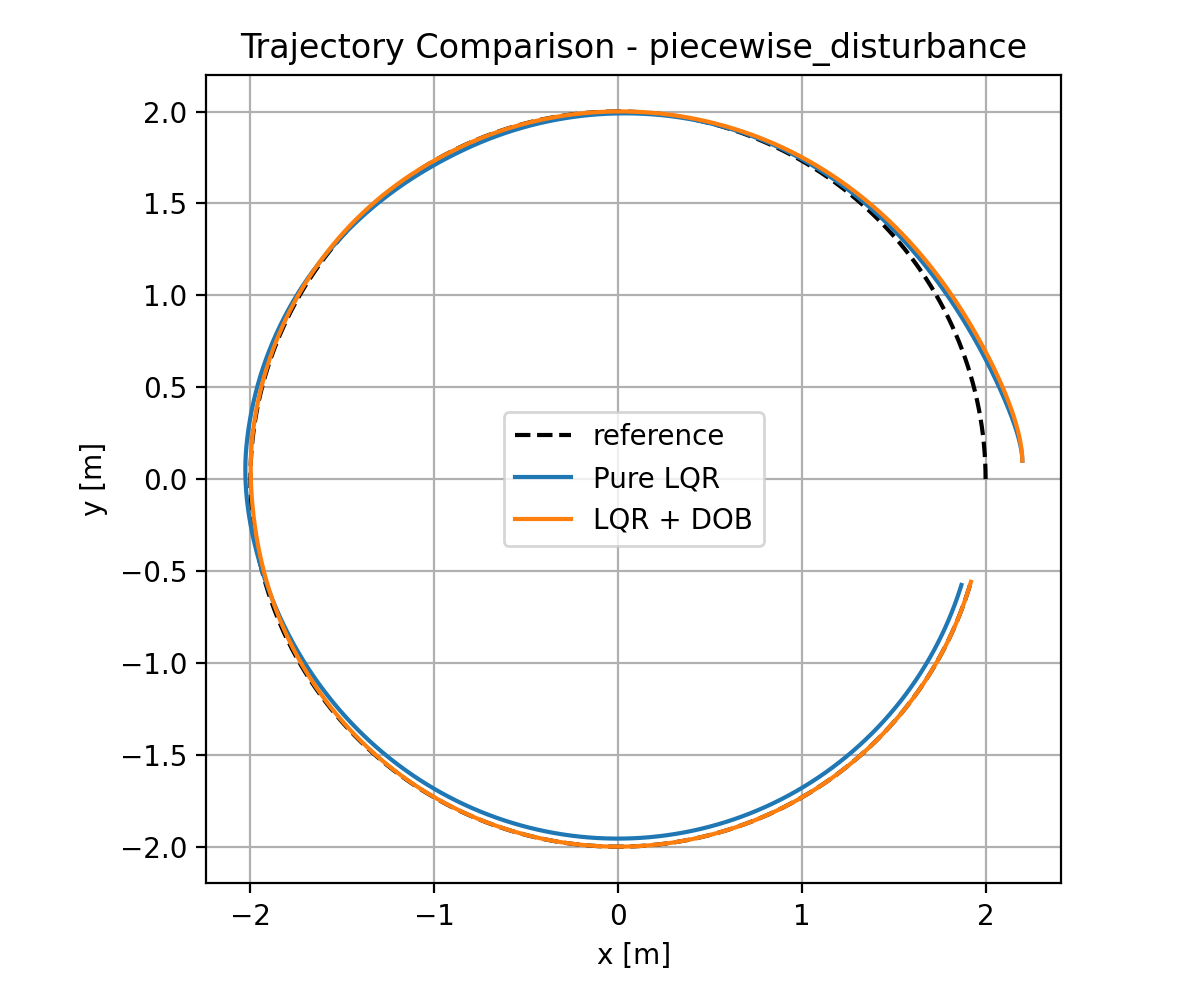
\includegraphics[width=\linewidth]{figs/piecewise_disturbance_trajectory_compare.png}
    \column{0.45\linewidth}
      \textbf{Observation}
      \begin{itemize}
        \item Both controllers visually track the reference
        \item LQR drifts slightly after each disturbance switch
              (lower arc)
        \item LQR+DOB stays within mm of the reference circle
      \end{itemize}

      \vspace{0.6em}
      Trajectory plot understates the difference — see error time
      series on the next slide.
  \end{columns}
\end{frame}

\begin{frame}{The key result: step disturbance position error (S2)}
  \begin{columns}[T]
    \column{0.55\linewidth}
      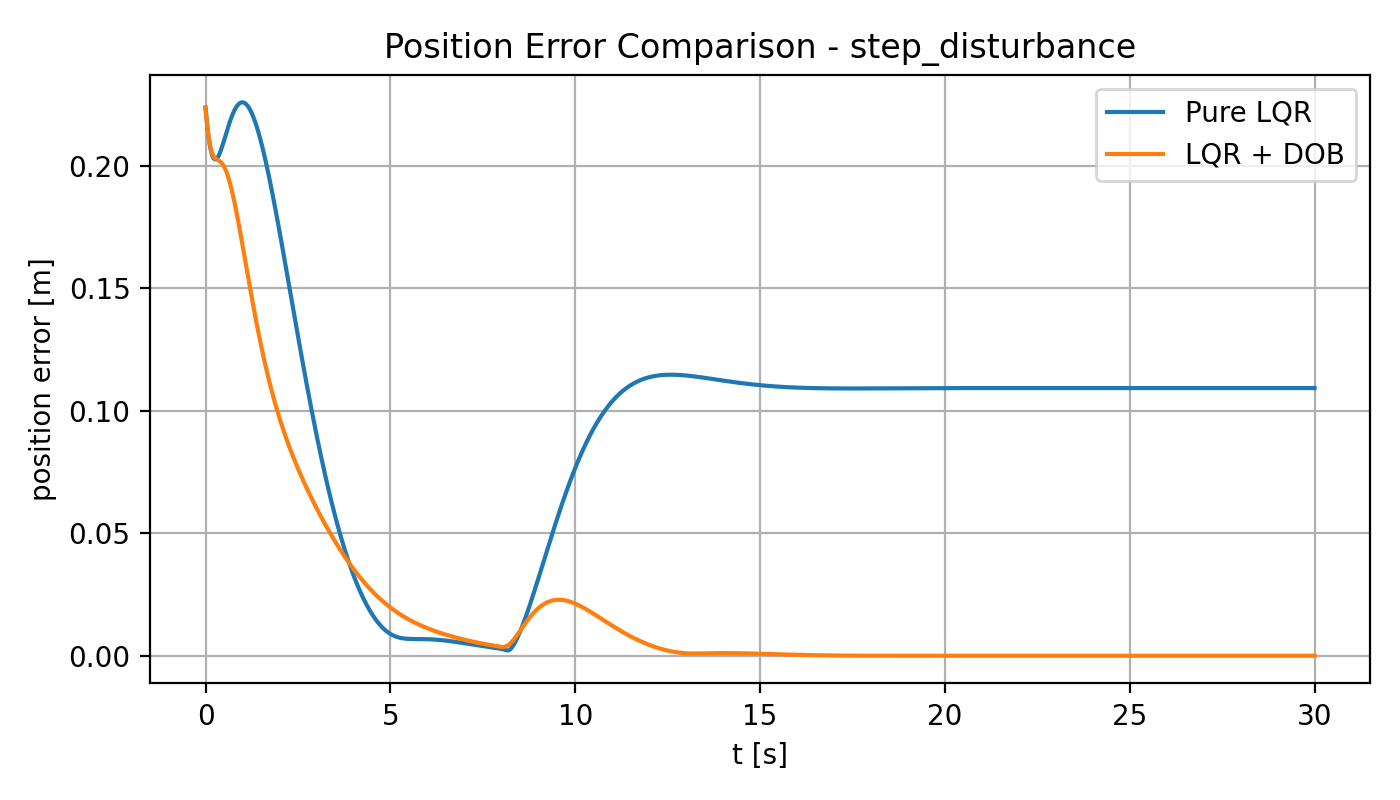
\includegraphics[width=\linewidth]{figs/step_disturbance_position_error_compare.png}
    \column{0.45\linewidth}
      \textbf{LQR (blue)}
      \begin{itemize}
        \item Initial transient decays as expected
        \item At $t=8$\,s: disturbance hits
        \item \alert{Settles at $\sim 0.11$\,m steady state}
      \end{itemize}

      \vspace{0.5em}
      \textbf{LQR+DOB (orange)}
      \begin{itemize}
        \item Same nominal transient
        \item Observer catches the disturbance in $\sim 4$\,s
        \item Recovers to zero error
      \end{itemize}

      \vspace{0.5em}
      \alert{This is the central observation of the project.}
  \end{columns}
\end{frame}

\begin{frame}{Disturbance estimate vs.\ truth (S3)}
  \begin{columns}[T]
    \column{0.55\linewidth}
      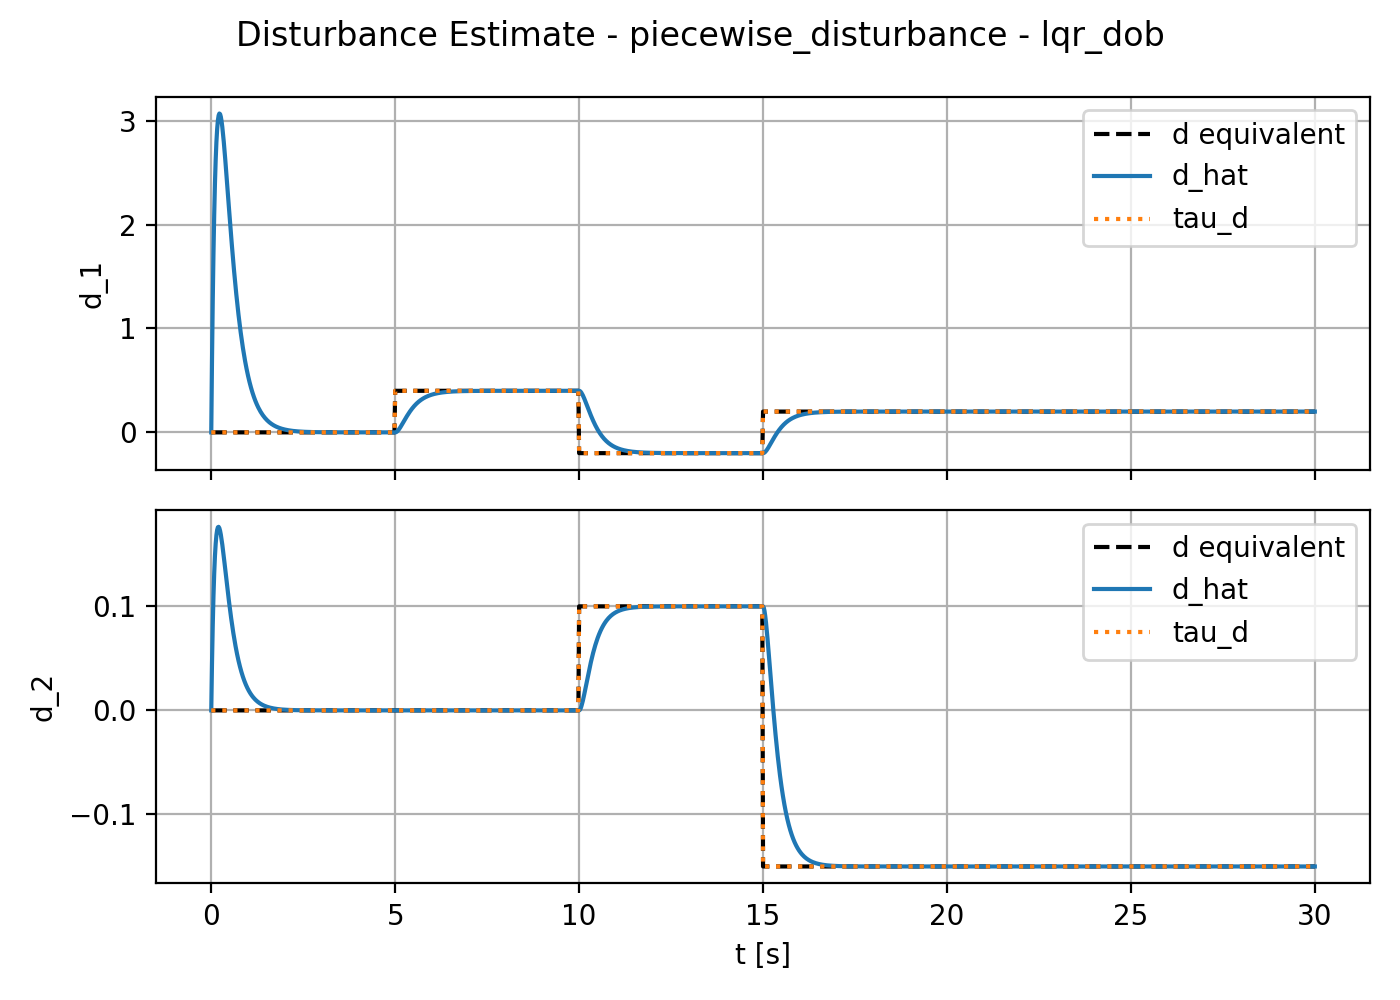
\includegraphics[width=\linewidth]{figs/piecewise_disturbance_d_hat.png}
    \column{0.45\linewidth}
      $\hat d$ tracks the \alert{equivalent matched disturbance}
      with $\approx 1/(\rho\alpha)\!\approx\!0.33$\,s lag.

      \vspace{0.6em}
      \textbf{Two components shown:}
      \begin{itemize}
        \item $d_1$: force-channel disturbance (top)
        \item $d_2$: torque-channel (bottom)
      \end{itemize}

      \vspace{0.4em}
      Initial spike at $t=0$ is the observer's own transient — predicted
      by Theorem 1.

      \vspace{0.4em}
      No bias in steady state — the observer's internal integrator
      eliminates DC error.
  \end{columns}
\end{frame}

\begin{frame}{Quantitative summary across all five scenarios}
  \centering
  \scriptsize
  \begin{tabular}{llcccc}
    \toprule
    Scenario & Controller & RMSE [m] & ITAE & Effort & Dist.\,RMSE\\
    \midrule
    \multirow{2}{*}{Nominal}      & LQR     & 0.0608 & 1.17  & 3.16  & ---\\
                                  & LQR+DOB & \textbf{0.0467} & \textbf{0.98}  & 7.83  & 0.370\\
    \midrule
    \multirow{2}{*}{Step}         & LQR     & 0.1084 & 45.42 & 9.14  & ---\\
                                  & LQR+DOB & \textbf{0.0471} & \textbf{1.57}  & 13.88 & 0.373\\
    \midrule
    \multirow{2}{*}{Piecewise}    & LQR     & 0.0775 & 22.83 & 5.14  & ---\\
                                  & LQR+DOB & \textbf{0.0476} & \textbf{2.99}  & 9.99  & 0.380\\
    \midrule
    \multirow{2}{*}{Payload}      & LQR     & 0.0610 & 1.72  & 3.18  & ---\\
                                  & LQR+DOB & \textbf{0.0467} & \textbf{1.05}  & 7.83  & 0.370\\
    \midrule
    \multirow{2}{*}{Noise+Fric}   & LQR     & 0.0932 & 27.86 & 6.78  & ---\\
                                  & LQR+DOB & \textbf{0.0475} & \textbf{2.94}  & 11.67 & 0.380\\
    \bottomrule
  \end{tabular}

  \vspace{0.6em}
  \normalsize
  \begin{itemize}
    \item RMSE under LQR+DOB \alert{stays in $[0.0467, 0.0476]$}\,m across all
          scenarios — DOB \emph{flattens} disturbance dependence
    \item ITAE reduced by \alert{up to a factor of 29} (Step)
    \item Cost: $\sim 2\times$ control effort
  \end{itemize}
\end{frame}

\begin{frame}{Observer-speed sweep $\rho\in\{2,3,5,8,12\}$ (S3)}
  \begin{columns}[T]
    \column{0.6\linewidth}
      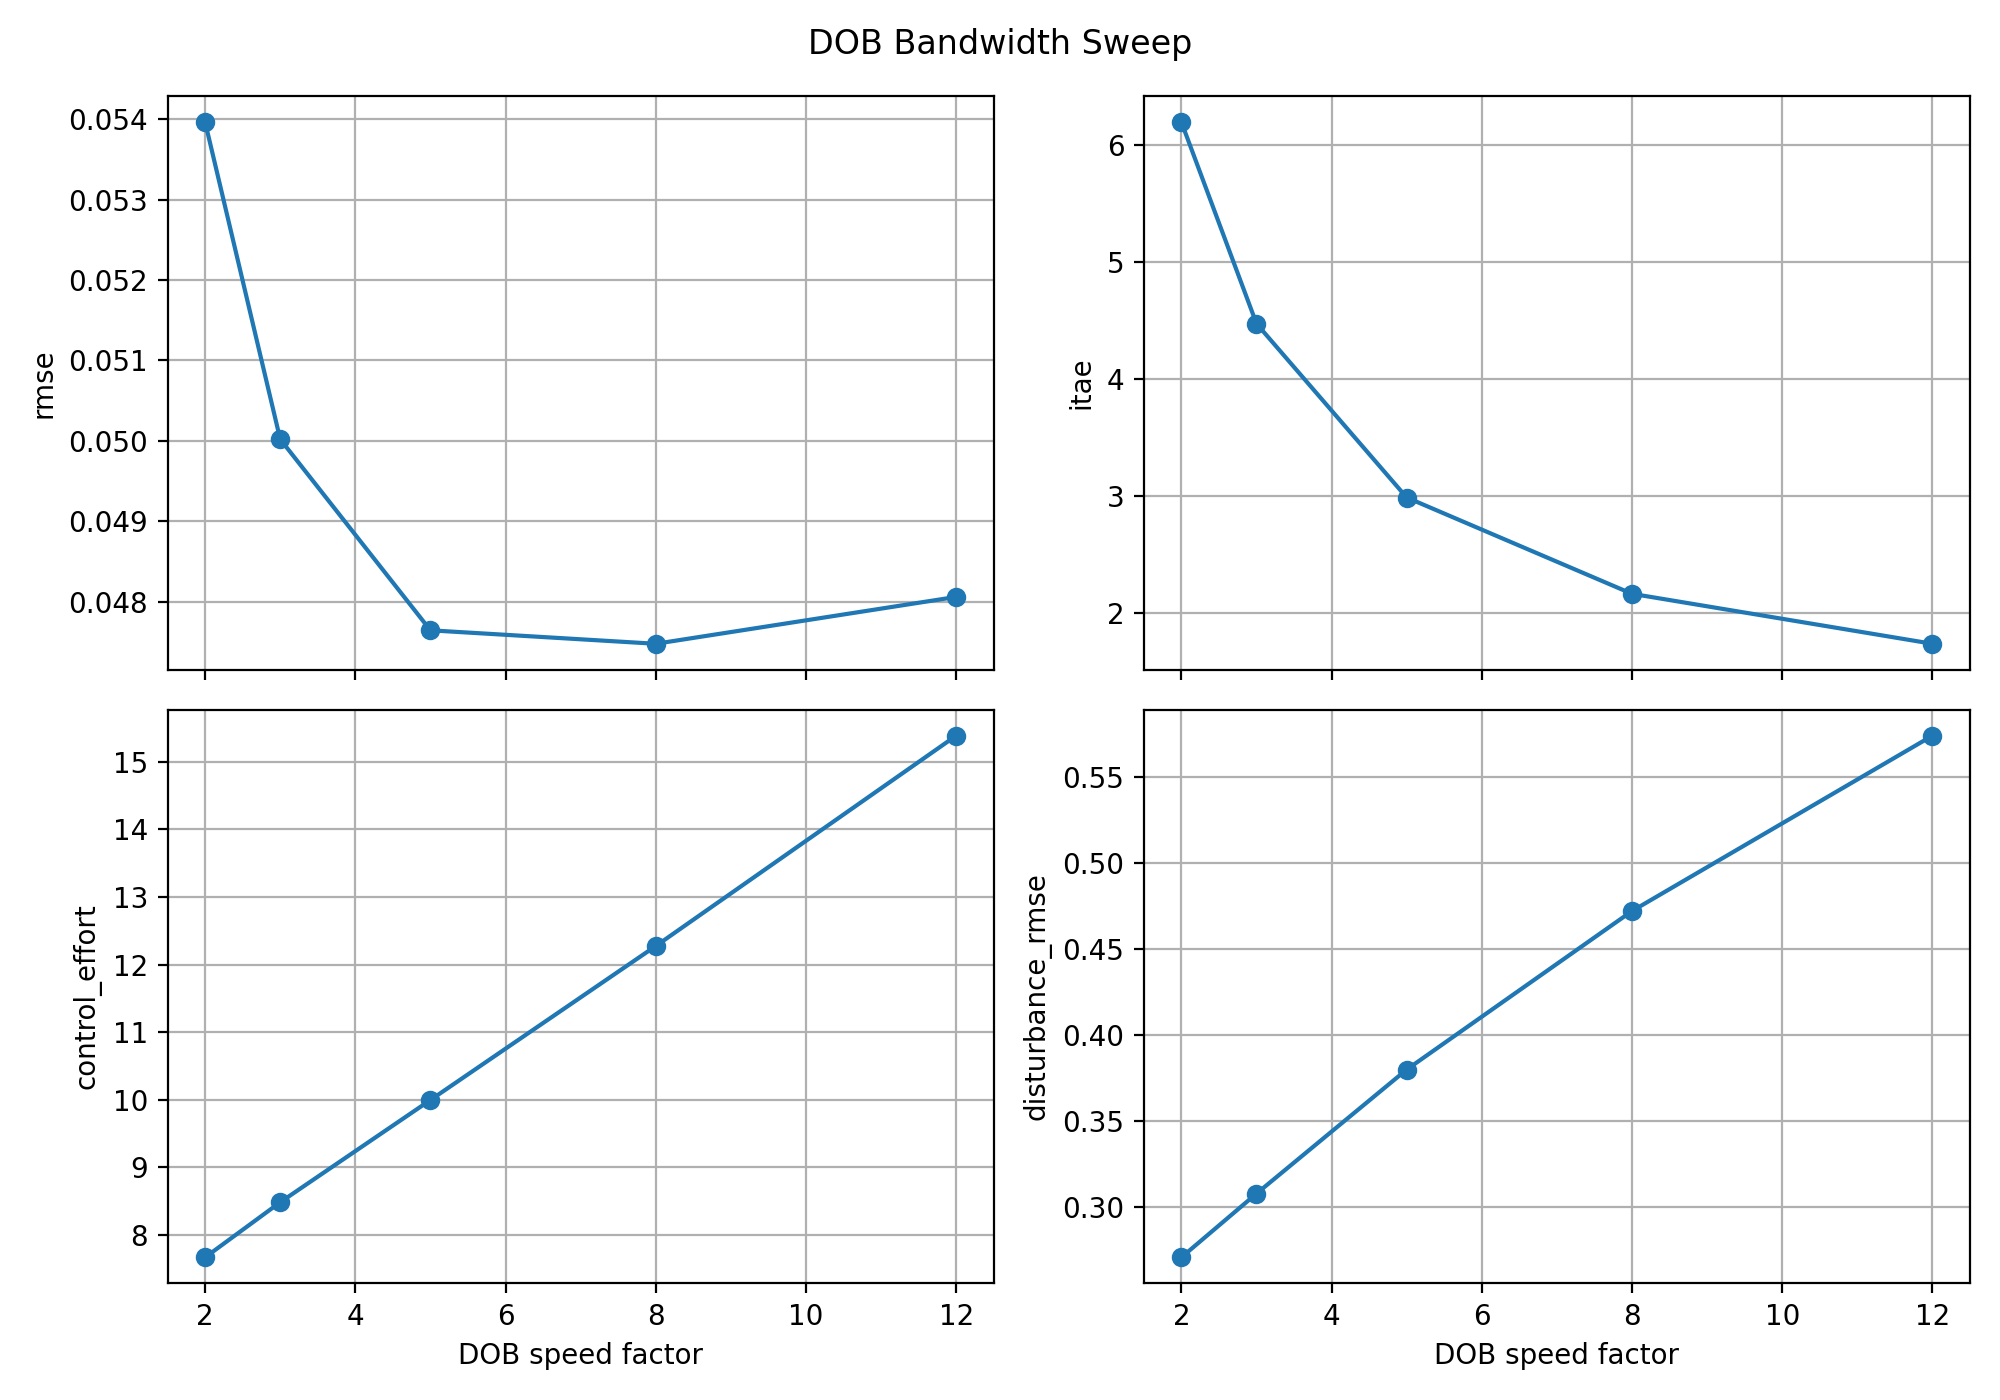
\includegraphics[width=\linewidth]{figs/dob_sweep.png}
    \column{0.4\linewidth}
      \textbf{Observations}
      \begin{itemize}
        \item RMSE bottoms at $\rho\!\in\![5,8]$
        \item ITAE \alert{monotonically} improves with $\rho$
        \item Control effort grows \alert{linearly}
        \item Disturbance-estimate noise also grows linearly
      \end{itemize}

      \vspace{0.6em}
      \textbf{$\rho=5$ chosen as default}:
      \begin{itemize}
        \item Near minimum RMSE
        \item Sub-3s ITAE
        \item $\sim 10$ effort units (reasonable)
      \end{itemize}
  \end{columns}
\end{frame}

%%%%%%%%%%%%%%%%%%%%%%%%%%%%%%%%%%%%%%%%%%%%%%%%%%%%%%%%%%%%%%%%%%%%%%%%%%%%%%%
\section{Conclusion}

\begin{frame}{Key take-aways}
  \begin{enumerate}\setlength\itemsep{0.6em}
    \item \textbf{LQR alone is brittle to persistent disturbance} —
          a $0.5$\,N$\cdot$m step gives 0.11\,m steady-state offset.
    \item \textbf{DOB cancels matched disturbance transparently} —
          RMSE collapses to near-nominal across \alert{all} 5
          uncertainty scenarios.
    \item \textbf{Parametric drift = matched disturbance.} Tripling
          the payload changes nothing for LQR+DOB.
    \item \textbf{Pole-placement rule with time-scale separation
          $\rho$} gives a clean, principled design:
          \begin{itemize}\setlength\itemsep{1pt}
            \item small $\rho$ $\Rightarrow$ ITAE penalty
            \item large $\rho$ $\Rightarrow$ noise / effort penalty
            \item $\rho\!\approx\!5$ is a sweet spot
          \end{itemize}
    \item \textbf{Stability is guaranteed} by a composite Lyapunov
          function — proof in Appendix B of the report.
  \end{enumerate}
\end{frame}

\begin{frame}{Limitations and future work}
  \begin{block}{Limitations}
    \begin{itemize}
      \item Only \emph{matched} disturbances are cancelled
      \item Constant-curvature reference (no path transitions)
      \item Simulation-only — no real-robot validation yet
    \end{itemize}
  \end{block}

  \begin{block}{Future work}
    \begin{itemize}
      \item Generalised extended state observer for polynomial $d$
            \cite{li2012generalized}
      \item Time-varying reference with curvature transitions
      \item Experimental validation on TurtleBot3 platform
    \end{itemize}
  \end{block}
\end{frame}

% ============================== Thanks ============================ %
\begin{frame}[standout]
  Thank you.\\[1em]
  \normalsize Questions?
\end{frame}

%%%%%%%%%%%%%%%%%%%%%%%%%%%%%%%%%%%%%%%%%%%%%%%%%%%%%%%%%%%%%%%%%%%%%%%%%%%%%%%
% References
\appendix

\begin{frame}[allowframebreaks]{References}
  \footnotesize
  \begin{thebibliography}{99}
    \bibitem{kanayama1990} Y.~Kanayama \textit{et al.},
      ``A stable tracking control method for an autonomous mobile robot,''
      \emph{ICRA}, 1990.
    \bibitem{klancar2007} G.~Kla\v{n}car and I.~\v{S}krjanc,
      ``Tracking-error model-based predictive control for mobile robots
      in real time,'' \emph{Rob.\ Auton.\ Syst.}, 2007.
    \bibitem{ohnishi1996} K.~Ohnishi \textit{et al.},
      ``Motion control for advanced mechatronics,''
      \emph{IEEE/ASME TMech}, 1996.
    \bibitem{chen2016} W.-H.\ Chen \textit{et al.},
      ``Disturbance-observer-based control and related methods,''
      \emph{IEEE TIE}, 2016.
    \bibitem{li2012generalized} S.~Li \textit{et al.},
      ``Generalized ESO for systems with mismatched uncertainties,''
      \emph{IEEE TIE}, 2012.
    \bibitem{kayacan2015} E.~Kayacan \textit{et al.},
      ``Robust trajectory tracking error model-based predictive control
      for UGVs,'' \emph{IEEE/ASME TMech}, 2015.
    \bibitem{utkin2013} V.~Utkin \textit{et al.},
      \emph{Sliding Mode Control in Electro-mechanical Systems},
      CRC Press, 2013.
    \bibitem{zhou1996} K.~Zhou \textit{et al.},
      \emph{Robust and Optimal Control}, Prentice Hall, 1996.
    \bibitem{mayne2005} D.~Q.\ Mayne \textit{et al.},
      ``Robust MPC of constrained linear systems with bounded
      disturbances,'' \emph{Automatica}, 2005.
    \bibitem{kautsky1985} J.~Kautsky \textit{et al.},
      ``Robust pole assignment in linear state feedback,''
      \emph{IJC}, 1985.
  \end{thebibliography}
\end{frame}

\end{document}
